\documentclass[format=acmsmall, review=false, screen=true]{acmart}

\usepackage{booktabs} % For formal tables

\usepackage[ruled]{algorithm2e} % For algorithms
\renewcommand{\algorithmcfname}{ALGORITHM}
\SetAlFnt{\small}
\SetAlCapFnt{\small}
\SetAlCapNameFnt{\small}
\SetAlCapHSkip{0pt}
\IncMargin{-\parindent}


% Metadata Information
\acmJournal{TWEB}
\acmVolume{9}
\acmNumber{4}
\acmArticle{39}
\acmYear{2010}
\acmMonth{3}
\copyrightyear{2009}
%\acmArticleSeq{9}

% Copyright
%\setcopyright{acmcopyright}
\setcopyright{acmlicensed}
%\setcopyright{rightsretained}
%\setcopyright{usgov}
%\setcopyright{usgovmixed}
%\setcopyright{cagov}
%\setcopyright{cagovmixed}

% DOI
\acmDOI{0000001.0000001}

% Paper history
\received{February 2007}
\received[revised]{March 2009}
\received[accepted]{June 2009}


% Document starts
\begin{document}
% Title portion. Note the short title for running heads 
\title[A Multifrequency MAC for Wireless Sensor]{A Multifrequency MAC
  Specially Designed for Wireless Sensor  Network Applications}  
\author{Gang Zhou}
\orcid{1234-5678-9012-3456}
\affiliation{%
  \institution{College of William and Mary}
  \streetaddress{104 Jamestown Rd}
  \city{Williamsburg}
  \state{VA}
  \postcode{23185}
  \country{USA}}
\author{Yafeng Wu}
\affiliation{%
  \institution{University of Virginia}
  \department{School of Engineering}
  \city{Charlottesville}
  \state{VA}
  \postcode{22903}
  \country{USA}
}
\author{Ting Yan}
\affiliation{%
  \institution{Eaton Innovation Center}
  \city{Prague}
  \country{Czech Republic}}
\author{Tian He}
\affiliation{%
  \institution{University of Minnesota}
  \country{USA}}
\author{Chengdu Huang}
\author{John A. Stankovic}
\author{Tarek F. Abdelzaher}
\affiliation{%
  \institution{University of Virginia}
  \department{School of Engineering}
  \city{Charlottesville}
  \state{VA}
  \postcode{22903}
  \country{USA}
}

\begin{abstract}
Multifrequency media access control has been well understood in
general wireless ad hoc networks, while in wireless sensor networks,
researchers still focus on single frequency solutions. In wireless
sensor networks, each device is typically equipped with a single
radio transceiver and applications adopt much smaller packet sizes
compared to those in general wireless ad hoc networks. Hence, the
multifrequency MAC protocols proposed for general wireless ad hoc
networks are not suitable for wireless sensor network applications,
which we further demonstrate through our simulation experiments. In
this article, we propose MMSN, which takes advantage of
multifrequency availability while, at the same time, takes into
consideration the restrictions of wireless sensor networks. Through
extensive experiments, MMSN exhibits the prominent ability to utilize
parallel transmissions among neighboring nodes. 
\end{abstract}


%
% The code below should be generated by the tool at
% http://dl.acm.org/ccs.cfm
% Please copy and paste the code instead of the example below. 
%
\begin{CCSXML}
<ccs2012>
 <concept>
  <concept_id>10010520.10010553.10010562</concept_id>
  <concept_desc>Computer systems organization~Embedded systems</concept_desc>
  <concept_significance>500</concept_significance>
 </concept>
 <concept>
  <concept_id>10010520.10010575.10010755</concept_id>
  <concept_desc>Computer systems organization~Redundancy</concept_desc>
  <concept_significance>300</concept_significance>
 </concept>
 <concept>
  <concept_id>10010520.10010553.10010554</concept_id>
  <concept_desc>Computer systems organization~Robotics</concept_desc>
  <concept_significance>100</concept_significance>
 </concept>
 <concept>
  <concept_id>10003033.10003083.10003095</concept_id>
  <concept_desc>Networks~Network reliability</concept_desc>
  <concept_significance>100</concept_significance>
 </concept>
</ccs2012>  
\end{CCSXML}

\ccsdesc[500]{Computer systems organization~Embedded systems}
\ccsdesc[300]{Computer systems organization~Redundancy}
\ccsdesc{Computer systems organization~Robotics}
\ccsdesc[100]{Networks~Network reliability}

%
% End generated code
%

% We no longer use \terms command
%\terms{Design, Algorithms, Performance}

\keywords{Wireless sensor networks, media access control,
multi-channel, radio interference, time synchronization}


\thanks{This work is supported by the National Science Foundation,
  under grant CNS-0435060, grant CCR-0325197 and grant EN-CS-0329609.

  Author's addresses: G. Zhou, Computer Science Department, College of
  William and Mary; Y. Wu {and} J. A. Stankovic, Computer Science
  Department, University of Virginia; T. Yan, Eaton Innovation Center;
  T. He, Computer Science Department, University of Minnesota; C.
  Huang, Google; T. F. Abdelzaher, (Current address) NASA Ames
  Research Center, Moffett Field, California 94035.}


\maketitle

% The default list of authors is too long for headers}
\renewcommand{\shortauthors}{G. Zhou et al.}


\section{INTRODUCTION}

Cryptographic algorithms are widely used in cryptographic systems and play a significant role.When we use cryptographic algorithms to implement cryptographic systems, we usually use existing Open Source cryptographic libraries to complete the required calculations and combine them with application functions.
The cryptographic software system is linked to the user's core interests. When users use online transactions, e-mail, and remote login services, they rely on the protection of cryptographic software systems. Once the security of cryptographic software systems is not guaranteed, it will cause extreme problems for users. Big losses; on the other hand, the speed of password computing directly affects the user's experience with the crypto software system. Therefore, it is imperative to provide secure, high-speed and reliable cryptographic services.
However, existing programs face various memory disclosure attacks and the security of sensitive data cannot be guaranteed, especially key security.We need a more principled approach to defense memory disclosure attacks.

%����peapods�ı�Ҫ��

\textbf{Memory Disclosure Attacks}

%��Ҫ�����ڴ�й©������������в
There are many security threats when the cryptographic algorithm is running. One of them is sensitive information stored in the memory, such as a key, which is stolen by an adversary.One of the attacks is a memory disclosure attack. Memory disclosure attacks are read-only memory attacks where the adversary can obtain the contents of the memory but cannot tamper with it. Memory disclosure attacks include software attacks and hardware attacks.Software attack means that the attacker does not physically touch the attack target. It uses software vulnerabilities to bypass the system protection mechanism and illegally accesses the data in the memory.Such as OpenSSL heart bleeding attack, using OpenSSL heartbeat vulnerability, so that remote attackers can obtain a server 64KB memory data by constructing a malicious request.Hardware attack means that an attacker can physically contact an attack target and use a physical method to read the memory of the target.Such as cold-boot attack, using the delay disappearance effect of DRAM, directly read the contents of the memory chip.In short, memory disclosure attacks pose a serious threat to plain-text sensitive data in memory.

Therefore, the sensitive data needs to find a secure temporary storage area so that it can be stored in clear text and can also be accessed by instructions in the cryptographic algorithm implementation.This secure temporary storage area should enable the sensitive information that needs to be protected when the cryptographic algorithm is run to be stored in clear text. The information out of this area needs to be encrypted and saved.There are two types of sensitive information that need to be protected: (1) Persistent sensitive information, such as a master key, is used to encrypt information leaving a secure area and decrypt information entering a secure area, (2) Non-persistent sensitive information, such as temporary data generated during the calculation that can be used to derive the key.For the master key, it is always stored in secure storage in clear text whether or not the sensitive information calculation is to be performed.The non-persistent sensitive information is generated when the master key is used to decrypt or calculate after the calculation starts. The plaintext is stored in the secure area. When the sensitive information calculation is completed, it is cleared from the secure area.

For physical memory attacks in memory disclosure attacks, any storage area that can restrict access only at the software level is insecure. Secure storage should have physical mechanisms to restrict access.Each CPU core or each hardware thread has a separate set of registers that can only be read by the currently executing instruction.Therefore, the register is the storage resource that runs the program exclusive and it is an ideal secure storage.

In addition, the transactional memory mechanism provides a suitable secure temporary storage area. Transactional memory mechanisms implemented with hardware, such as TSX, can effectively defend against physical memory attacks.
%�����ڴ�����ṩ�˺��ʵİ�ȫ�洢����ʹ��Ӳ������ʵ�ֵ������ڴ���ƣ���TSX��������Ч�ط���physical memory attacks

\textbf{Peapods}
%����peapods����

Peapods is a compiler enhancement tool that provides security enhancements for cryptographic software systems that can defend against software memory attacks and cold-boot attack when programmers using the Open Source cryptographic library.

In our scenario, a Peapod represents a protected key-related calculation (especially the private key calculation in the public-key cryptographic algorithm).Through the transactional memory mechanism, we can guarantee that in the course of calculation, once an attacker reads the key, the key will be automatically cleared.If the computing key is in a non-calculated state, it is in a ciphertext state.Further, to ensure that calculations can be completed in the transactional memory protection state, it can be split into multiple partitioned tasks.Between the partitioned tasks will exit the transactional memory state, but the calculated intermediate variables will also be encrypted to avoid the leakage of sensitive information.

%Peapods can automatically encrypt and decrypt sensitive variables when users add a small amount of code. Therefore, we can provide security enhancements for various types of cryptographic software systems without the need to reconstruct the entire cryptographic software system and add a small amount of source code in the presence of security vulnerabilities. On the platform supporting Intel TSX features, we implemented the Peapods prototype based on the transactional memory mechanism, and through simulated attacks, we proved that Peapods can effectively prevent malicious code from accessing sensitive information. Moreover, compared to Polar SSL protected by Peapods and non-protected Polar SSL, the performance loss is only 10\% within an acceptable range.

\textbf{Implementation}
%ʵ��

We implemented Peapods in LLVM for x86 and recompiled PolarSSL and all of its dependencies.We use Peapods to protect Polarssl RSA decryption calculations and users only need to make a few code changes(less than 1000 lines).Experiment shows that compared to PolarSSL protected by Peapods and non-protected PolarSSL, the overhead is only 10\% within an acceptable range.
% Head 1
\section{BACKGROUND}

\subsection{Memory Disclosure Attacks}
\textbf{physical memory attack}

Physical memory attack refers to the behavior of the attacker directly reading the memory chip and obtaining the data illegally after the attacker has physical control over the attack target.In this case, any software-based protection will fail because the attacker can directly manipulate the hardware.Physical memory attack mainly include two types: (1)cold boot attack, which uses DRAM's delay-disappearing effect to directly read the contents of the memory chip, (2)DMA attack, which initiate illegal DMA requests through malicious peripherals, and directly read data from the memory chip.

\textbf{software memory attack}

Software memory attack refers to the behavior of the attacker does not physically contact the attack target, and uses software vulnerabilities to bypass the system protection mechanism and illegally access the data in the memory.For example, OpenSSL heart bleeding attack exploits the vulnerability of OpenSSL heartbeat to enable remote attackers to obtain 64KB of memory data from the server once by constructing a malicious request.Software memory attack mainly include four types: (1)attack based on an isolation mechanism vulnerability, which exploits the defect of the virtual memory subsystem of the operating system to illegally access data from the memory chip, (2)attack based on unclear dynamic memory, which originates from the fact that the dynamic memory storing sensitive information is not cleared and is used by other programs, (3)attack based on cryptographic software's own vulnerability, such as OpenSSL heart bleeding attack, (4)attack based on memory data diffusion, which exploits normal operating system functionality.For example, kernel dumps were originally used to save memory images to disk for developers to debug after a software crash, but attackers can also use this feature to deliberately trigger an exception that causes the software to crash, and then read the sensitive data contained in the process from the disk.

These types of attacks pose a great threat to users' sensitive data.We need a complete solution to defend against these attacks and protect users' data security.
%ö���ڴ�й©��������

\subsection{TSX}
%TSX and RTM
%���������ڴ��RTM�ӿ�
Transactional memory is a software technique that simplifies writing concurrent programs.The main idea is to declare a region of code as a transaction. A transaction executes and atomically commits all the results to memory when the transaction succeeds or aborts and cancels all the results if the transaction fails. Transactional memory mechanism provide the Atomicity, Consistency and Isolation qualities. These transactions can safely execute in parallel, and only serial execution is performed in the case of data conflicts, which happen when several threads access the same memory address at the same time and at least one is write operation.When a data conflict occurs, it will cause a rollback and all the results will be canceled.

The recent development is Intel��s TSX and the implementation in Haswell.Haswell is the first x86 processor to feature hardware transactional memory.Programmers only need to specify
critical sections for transactional executions, the processor transparently performs data conflict detection, transaction commit and rollback.TSX tracks the read-set and write-set of a transaction, at a 64B cache line granularity. The read-set and write-set are respectively all the cache lines that the transaction has read from, or written to during execution. A transaction encounters a conflict if a cache line in its read-set is written by another thread, or if a cache line in its write-set is read or written by another thread.

TSX provides two interfaces for programmers to make use of transactional memory. The first mode is Hardware Lock Elision(HLE), provides a pair of compiler hints:xacquire and xrelease to enter or exit the critical section.Once abort happens, the processor will roll back to the original state, and then automatically restarts the execution in a legacy manner. The second mode is Restricted Transactional Memory (RTM), provides three new instructions, XBEGIN, XEND and XABORT, to start, commit, and abort a transactional execution.When using the RTM interface, the programmer needs to specify a fallback handler for the XBEGIN instruction as a parameter and write the fallback handler logic. When a transaction aborts, the program jumps to the specified fallback handler and executes the corresponding program logic.
\subsection{LLVM}

LLVM is an abbreviation of low level virtual machine. It is actually a compiler framework. With the continuous development of this project, llvm has been unable to fully represent this project, but this name has been continued, and it can now be understood as a full-featured compiler. LLVM can be seen as a collection of compiler and toolchain technologies, and they are modular and reusable.

The traditional compiler is divided into front-end, optimizer, back-end three stages, llvm is also divided into three stages, but slightly different in the design.

Because LLVM is a virtual machine, it has its own Intermediate Representation. It needs to compile the LLVM byte code into a platform-specific assembly language before it can be run by the native assembler and linker to generate assembly code, executable shared libraries, etc.

The front end fetches the source code and then turns it into an intermediate byte code representation.This translation simplifies the work of other parts of the compiler so that they do not need to deal with all the complexity of C++ source code.

In LLVM Optimizer, PASS transforms the program between the intermediate representation.In general, the process is used to optimize the code, that is, the process output program is completely functionally identical to its input program, but the performance is improved.However, we can also add code logic by adding an IR PASS to achieve a functional improvement over the input program.LLVM provides a lot of APIs for manipulating intermediate bytecode representations, so we can use these interfaces to generate IR directly in memory and run directly to achieve programmatic changes.The intermediate representation of the source code can be further divided into modules, functions, basic blocks, and instruction four-layer structures.

The back-end part translates the intermediate representation into the assembly language of the target platform and generates the actual running machine code.

Our work is to modify the intermediate representation of the source code through a Module PASS during the LLVM optimizer stage, adding logic such as generating a master key, identifying sensitive variables, and encrypting and decrypting sensitive data variables (unlike other situations. At this time, the program output by the process has changed in function compared with the program it has input), which enables the program to automatically protect the identified sensitive data variables and prevent the leakage of sensitive data information.
%\section{ THREAT MODEL AND security goals}





\section{DESIGN}


\subsection{ THREAT MODEL AND security goals}


In this paper we assume a powerful attacker who has the ability
to read arbitrary areas of memory and overwrite all writable
areas of memory. However, the attacker is unable to write to executable
memory (marked read-only) or read the value of special
registers our compiler reserves.

Peapods is focused on protecting user-level programs such as PolarSSL RSA decryption calculation, and we do not address protecting the kernel in this paper.
We assume that the kernel does not save any user-level registers��
at least the ones that are used to store the key��during context
switches in user accessible memory. This is true of all major modern
operating systems that we are aware of. Custom user-level
threading libraries may also require changes to ensure these registers
are not saved.

%��ϸ�ο�CCFI�İ�ȫģ�� dump�ڴ��������ν��з���
1.We assume that HTM is correctly implemented.

2.We assume that the integrity of the operating system kernel can be guaranteed.

3.We assume that the attacker cannot access the master key stored in the XMM7 register by executing the attack code.The attacker first needs to destroy the integrity of the control flow, there are currently many schemes that use the hardware lock mechanism to implement the control flow integrity.

4.We assume that the attacker has the ability to read data in memory, so we need to ensure that the master key stored in the XMM7 register is not leaked to memory. We modified the LLVM compilation, setting the XMM7 register as a reserved register, the LLVM compiler ensures that the code cannot control the reserved register. At the same time, we also modify the user-level threading libraries to prevent these registers been saved

%Ϊ�˵ֿ��ڴ�й©���� ���������ڴ湥��������������
%Ӧ�ò��������������ϵͳ�޹�

%ʵ�ֵ�peapods��һ������������  ʵ����X�Զ���X����
We proposes Peapods, a LLVM-based compiler enhancement tool that automates the protection of sensitive information in memory

%\section{CHALLENGES AND SOLUTIONS}
%1.�����Դ����Ļ�����ʵ�ֶ����б�����ʶ��ͼӽ��ܱ���
%LLVM PASS

%2.��ν���жϵ��µ�����abort����
%������

%3.��ν��ȱҳ����
%preloadԤ����

\subsection{ Structure of Peapods }
%\subsection{CHALLENGES AND SOLUTIONS}

%peapodsΪ���ܹ��ֿ��ڴ�й©����
Peapods is a LLVM-based compiler enhancement tool that protects memory that stores sensitive information.
%The basic idea is to apply HTM to protect the data in the transaction.
In our scenario, a Peapod represents a protected key-related calculation (especially the private key calculation in the public-key cryptographic algorithm).Through the transactional memory mechanism, we can guarantee that in the course of calculation, once an attacker reads the key, the key will be automatically cleared.If the computing key is in a non-calculated state, it is in a ciphertext state.Further, to ensure that calculations can be completed in the transactional memory protection state, it can be split into multiple partitioned tasks.Between the partitioned tasks will exit the transactional memory state, but the calculated intermediate variables will also be encrypted to avoid the leakage of sensitive information.

In order to achieve security goals,we divide the operation process of Peapods into three phases:User processing phase, Tool processing phase, Program execution phase

User processing phase:For sensitive variables whose compile-time address has already been determined, the user needs to add the keywords we provide in the place where the sensitive variables are defined. For sensitive variables whose compile-time address is not determined, the user needs to provide information of such sensitive variables,and then they also need to use the interface we provided for parameter passing through specified structure.When it is necessary to assign a value to a sensitive variable, the user needs to call START(args list) before the sensitive variable assignment and END(args list) after the assignment.
%peapods�������̷�Ϊ�û������׶Σ����ߴ����׶��Լ�����ִ�н׶�
%�û������׶Σ����ڱ���ʱ��ַ�Ѿ�ȷ�������б������û���Ҫ�����б�������ĵط����������ṩ�Ĺؼ��֣����ڱ���ʱ��ַδȷ�������б������û���Ҫ�ṩ�������б�������Ϣ��Ȼ��
%�ڶ�̬�⺯����ͨ��ָ���ṹ�崫��
%����Ҫ�����б������и�ֵʱ���û���Ҫ�����б�����ֵ֮ǰ����START
%��args list�����ڸ�ֵ֮�����END��args list����

Tool processing phase:1.Add initialization logic.2.For sensitive variables whose compile-time address has already been determined, Peapods recognizes variables that have been marked as sensitive data. If it is a local variable, it inserts the XBEGIN instruction before the instruction it defines, and other instructions after the next instruction of its defined instruction, including: (1) Use the master key to perform the CBC mode AES encryption of the intermediate byte code for the variable, and (2) the XEND instruction. Therefore, when these local variables are initialized in the way defined, the sensitive variables are stored in ciphertext in memory. Before the XEND instruction, Peapods will carefully clear the intermediate states used in this stage; If it is a global variable, the AES encryption of the CBC mode of all recognized global variables is completed at the time of program initialization.3.Peapods automatically encrypts and decrypts all sensitive variables in the structure for sensitive variables whose compilation addresses are undetermined.4.START,END, TEM function also adds automatic encryption and decryption protection logic
%���ߴ����׶Σ�
%1.���ӳ�ʼ���߼�
%2.���ڱ���ʱ��ַ�Ѿ�ȷ�������б�����Peapods����ѱ��Ϊ�������ݵı�������ʶ������Ǿֲ�������������䶨���ָ��֮ǰ����XBEGINָ����䶨���ָ�����һ��ָ��֮����룺��1��������Կ�Ըñ�������CBCģʽ��AES ���ܵ�
%�߼����м��ֽ��룬��2��XEND ָ���ˣ�����Щ�ֲ������Զ���ʱ��ʼ���ķ�ʽ���и�ֵ�Ļ������б����ͻ������ĵ���ʽ�������ڴ��У���XENDָ��֮ǰ��Peapods �Ὣ�ý׶����õ����м�״̬��С�ĵ���
%���������ȫ�ֱ���������ڳ����ʼ��ʱ��ɶ�������ʶ���ȫ�ֱ�����CBCģʽ��AES���ܡ�
%3.���ڱ���ʱ��ַδȷ�������б�����Peapods���Զ��Խṹ���е��������б������мӽ��ܱ�����
%4.START,END,TEMҲ�������Զ��ӽ��ܱ������߼�

%����ִ�н׶�
%��Ϊ��ʼ���׶Σ����б�������͸�ֵ�׶Σ���������׶�
Program execution phase:We can divide the program execution phase into initialization phase, sensitive variable definition and assignment phase, and protection calculation phase.

We use an AES master key to protect user sensitive data. The AES master key is generated at program startup and is then stored in the XMM7 register.Sensitive variables are AES encrypted after user-defined initialization or after assignment. When receiving a request for calculating sensitive information, Sensitive information is dynamically generated, used, and destroyed in transaction execution.When there is no computing task, sensitive information is always stored in ciphertext in memory.


%\begin{figure*}[!htb]
%\centering
%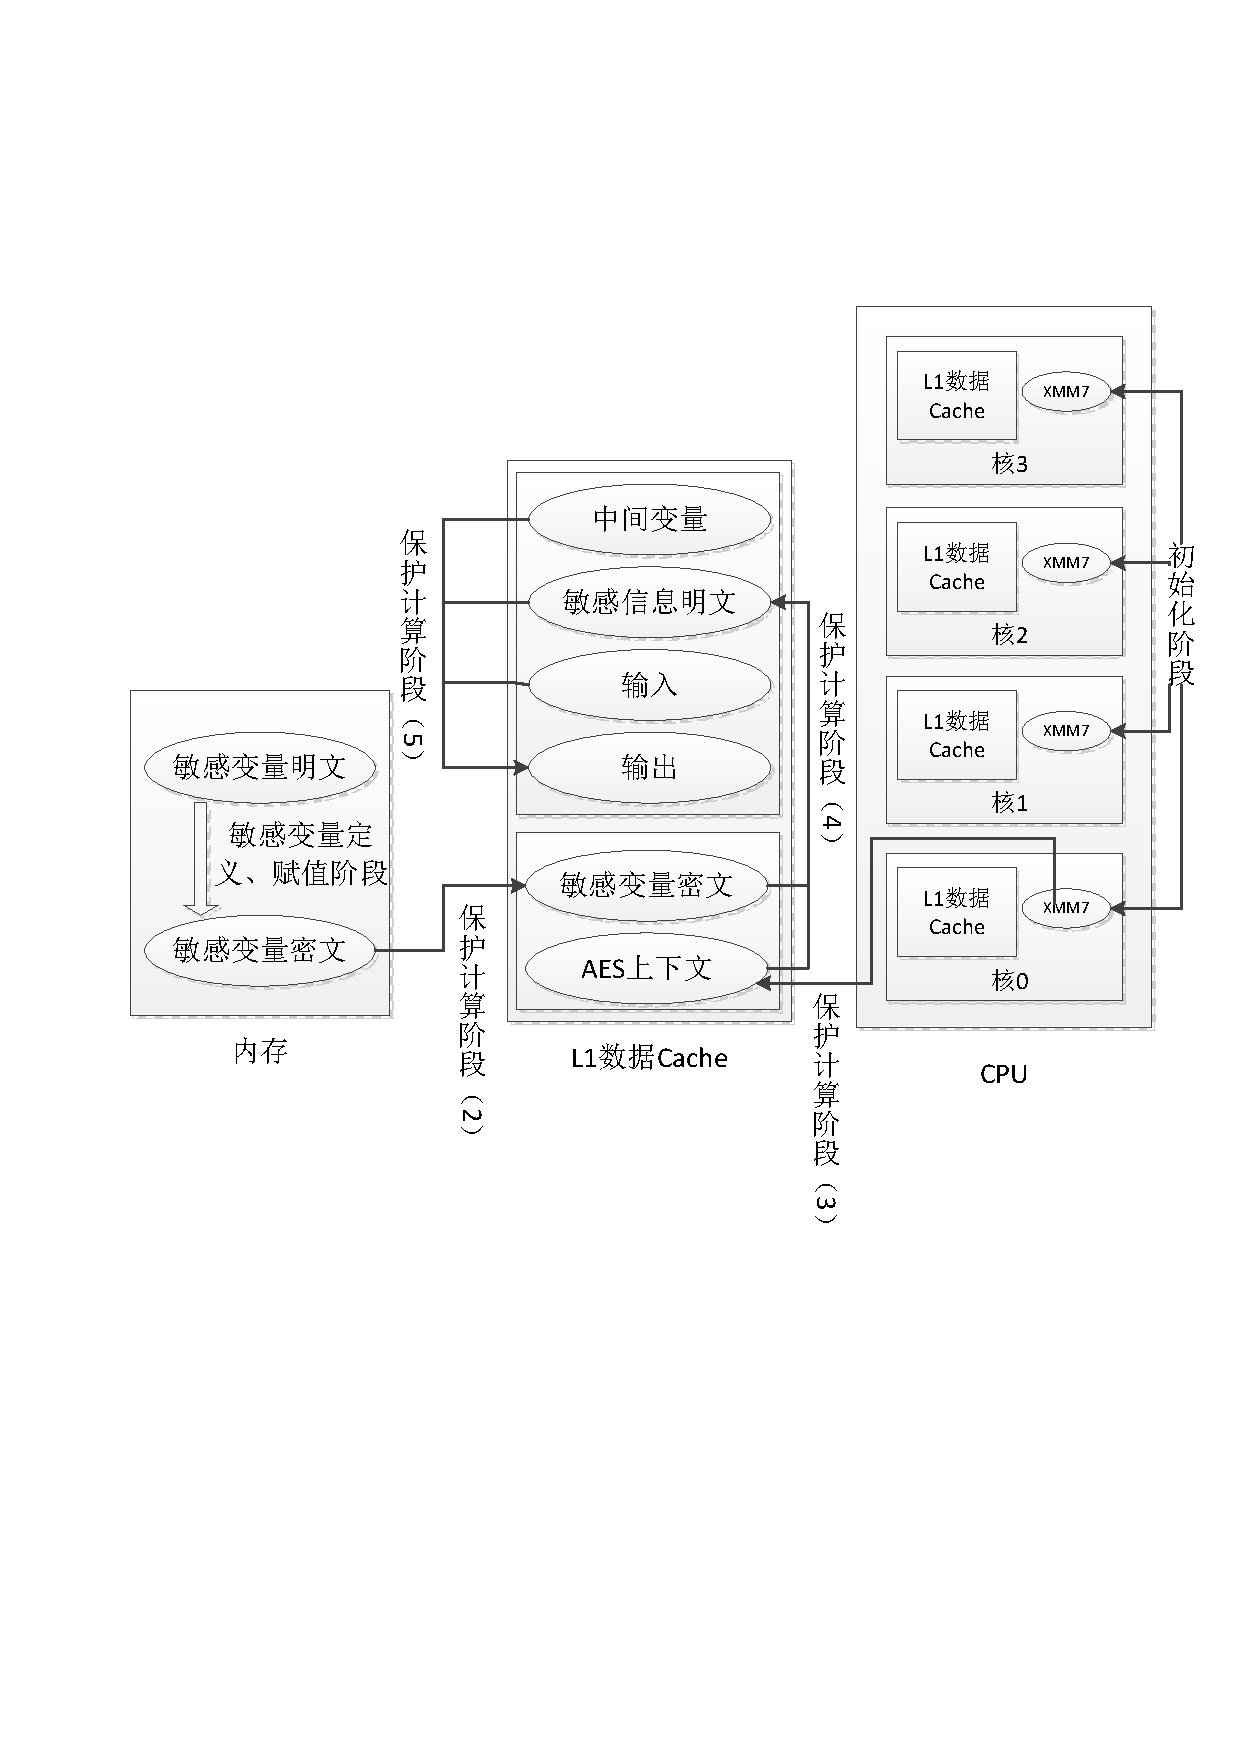
\includegraphics[width=0.9\textwidth]{design.pdf}
%\caption{Peapods����ܹ�}
%\label{fig:design}
%\end{figure*}

Initialization phase:
This stage starts when the program starts, mainly performing the following steps:
1.Randomly generate the AES master key and copy it to the XMM7 register in each CPU core.
2.Call the main function's preload function.
3.Call memset and other library functions.
4.The global variable IV is randomly generated, and the CBC-mode AES encryption is performed on all the global variable-sensitive information that has been identified.Finally, the intermediate states used in this phase are carefully cleared.

The first step is to generate the master key; the second and third steps are to prevent Peapods from abort the transaction due to page fault in the code segment; the last step is to store the sensitive information in ciphertext in memory.

Sensitive variable definition and assignment phase:
When the user needs to add a sensitive variable definition and assign value to the sensitive variable, Peapods encrypts the sensitive variable in plain text using the AES master key, so that the sensitive variable is stored in memory in ciphertext form.

Protection calculation phase:
When Peapods receives a sensitive information calculation request, sensitive information is calculated using the corresponding sensitive information, and then the result is provided to the user.This stage contains the following steps:
1.TSX begins to track memory access in the L1 data cache (maintaining read/write sets).
2.Ciphertext sensitive information is loaded into cache from memory.
3.Master key is loaded into cache from XMM7 register.
4.Use master key to decrypt sensitive information.
5.Calculation.
6.Clear all sensitive information in the cache and registers except the final calculation.
7.Commit transaction

All memory accesses in Protection calculation phase are monitored by hardware. In particular, we use Intel TSX technology to declare a transaction area in which operations that violate the security principles of Peapods are discovered: (1) Any attempt to access changed memory, because the decrypted plaintext Sensitive information and any private intermediate results are in the TSX write set; (2) Data is synchronized from cache to memory due to cache reclaim or replacement

If the above memory exception does not occur, the entire transaction is committed and the results are returned.Otherwise, the hardware's termination processing logic automatically discards all updated memory and then performs a rollback handler to handle the exception.We will immediately retry sensitive information calculations


\section{IMPLEMENTATION}
Our system is a C/C++ compiler built on the Clang/LLVM compiler framework. Any application wishing to be protected by Peapods must be recompiled along with all of its dependencies.

The LLVM module pass provides the sensitive variable identification logic, sensitive information encryption and decryption logic we need.

\subsection{Utility functions}


We encapsulate the XBEGIN and XEND instructions in user mode into utility functions START and END.They are used to start transactions and end transactions respectively.In addition,We also encapsulate an Utility functions TEM to split transactions.

%����ͼ
\subsection{Master key protection}
The master key needs to be saved in the system for a long time.The master key must be tightly protected, otherwise it will pose a threat to data security throughout the system.As persistent sensitive information, the master key is always stored in secure storage in clear text whether or not the sensitive information calculation is to be performed.For physical memory attacks in memory disclosure attacks, any storage area that can restrict access only at the software level is insecure. Secure storage should have physical mechanisms to restrict access.Each CPU core or each hardware thread has a separate set of registers that can only be read by the currently executing instruction.Therefore, the register is the storage resource that runs the program exclusive and it is an ideal secure storage. At the same time, XMM registers are mainly used for floating point and vector operations. Excluding a small number of XMM registers does not have a significant impact on performance in non-massive floating point computing environments.Therefore, we decided to store the master key in the XMM register.

The master key is randomly generated by the rdrand instruction at program startup.Then it is stored in the XMM7 register without any memory operations.In the LLVM backend, we set the XMM7 register as a reserved register.At last,user-level threading libraries have also made corresponding changes to prevent the value of XMM7 register from leaking into memory.
%rdrandָ����������
%�������ֱ�Ӳ����Ĵ�����û���漰�ڴ����
%XMM�Ĵ�������Ϊ�����Ĵ���
%user-level threading libraries Ҳ������Ӧ�ĸĶ�������Щ�Ĵ�����ֵй©���ڴ�


\subsection{sensitive variables Identification}

%4�ֲ�ͬ������ʶ��ͱ���
We divided the sensitive variables into two categories: (1) The address was already determined at compile time; (2) The address was not determined at compile time.
For sensitive variables whose compile-time addresses have been determined, such as sensitive variables for array types, structure types (members without pointer-type variables), we provide the user with the keyword: attribute ((annotation "Private Key")) when the user defining a sensitive data variable of this type, they need to add the keyword to the variable definition.Peapods will identify the variable that has been marked as sensitive data. If it is a local variable, it inserts the XBEGIN instruction before the instruction it defines, and inserts the instruction following its defined instruction: (1)The intermediate byte code of the logic of use the master key pair to encrypt this variable with AES encryption of the CBC mode, and (2) the XEND instruction.Therefore, when these local variables are initialized in the way defined, the sensitive variables are stored in ciphertext in memory. Before the XEND instruction, Peapods will carefully clear the intermediate states used in this stage;If it is a global variable, the AES encryption of the CBC mode of all recognized global variables is completed at the time of program initialization.

For sensitive variables with undecided compile-time addresses, such as pointer-type sensitive variables, since the address and length of sensitive variables cannot be obtained at compile time, the user is required to provide information of such sensitive variables. Then, the user uses the specified structure passes the parameters in the utility function provided by us, and Peapods will automatically encrypt and decrypt all the sensitive variables in the structure.

%�ṹ�����

\lstset{
    numbers=left,
    numberstyle= \tiny,
    keywordstyle= \color{ blue!70},
    commentstyle= \color{red!50!green!50!blue!50},
    frame=shadowbox, % ��ӰЧ��
    rulesepcolor= \color{ red!20!green!20!blue!20} ,
    escapeinside=``, % Ӣ�ķֺ��п�д������
    xleftmargin=2em,xrightmargin=2em, aboveskip=1em,
    framexleftmargin=2em
}
\begin{lstlisting}
struct args{
    unsigned char *data;
    int len;
    struct args* next;
}*args_list,args_list_next;
\end{lstlisting}

When users want to assign values to sensitive variables, they need to call START(args\_list) before assigning sensitive variables and END(args\_list) after assigning values.In IR PASS, we add logic to automatically encrypt and decrypt sensitive variables in utility functions such as START and END. In this way, the entire assignment process is performed under transaction protection. After the transaction is started, the sensitive variables are decrypted, and then encrypt sensitive variables before ending the transaction. Therefore, there is always only a ciphertext sensitive variable in memory.

It is worth noting that reading and writing files within a transaction will cause the transaction to abort. Therefore, Peapods cannot provide security protection during the assignment phase if the user reads a file to assign sensitive variables.In fact, in this case, the user can still call START(args list) after reading the file, call END(args list) after assignment, and clear the plaintext intermediate variable to make the sensitive variable exist in ciphertext after the assignment.However, in the process of reading a file, sensitive information is exposed in memory in the form of clear text. It is assumed that there is no memory disclosure attack at this time.At the same time, there is a backup of sensitive information in the hard disk. An attacker can also read the hard disk to obtain sensitive information. The user needs to delete the file containing sensitive information after reading the file.

\subsection{Sensitive information protection}
We provide users with three utility functions, and users call these utility functions as needed.We track all function call instructions in IR PASS, recognize the call to START, END, and TEM. Then we insert the corresponding intermediate representation code of encryption and decryption before the END function call instruction, after the START function call instruction, and both before and after the TEM function call instruction respectively.

\begin{table}[htbp]
 \caption{\label{tab:libfunc} Utility functions list}
 \centering
 \begin{tabular}{|c|c|p{3cm}<{\centering} | p{5cm}<{\centering} |}
  \toprule
  function name & function & usage method & Implementation logic \\
  \midrule
  START(args\_list) & Start a transaction & Used before sensitive operations begin & (1)XBEGIN��(2)get the master key from the XMM7 register��(3)generate AES context using the master key��(4)AES decryption of CBC mode for identified sensitive data variables \\
  \midrule
  END(args\_list) & End a transaction & Used after sensitive operations end & (1)AES encryption of CBC mode for identified sensitive data variables��(2)Erase intermediate results��(3)XEND \\
  \midrule
  TEM(args\_list) & Split a transaction & Used in locations where transactions need to be split within the transaction & (1)AES encryption of CBC mode for identified sensitive data variables��(2)Generate intermediate variable IV, then randomly initialize and perform AES encryption of CBC mode for the intermediate variables passed in by the user.��(3)Erase intermediate results��(4)XEND��(5)XBEGIN��(6)get the master key from the XMM7 register��(7)generate AES context using the master key��(8)AES decryption of CBC mode for identified sensitive data variables \\
  \bottomrule
 \end{tabular}
\end{table}
%�������ܺ����ľ���ʵ��ϸ�ڱ�
\subsection{Page fault handling}
We protected Polarssl RSA decryption calculations with peapods, during the execution of the program, we used perf, a performance analysis tool to help us knowing the program's operating status. Perf relies on the Intel performance monitoring facility, which supports precision-event-based sampling. This function can record the current processor state when a specific event occurs.We monitored the RTM\_RETIRED.ABORTED event, which was triggered when RTM execution was terminated.Based on the processor status acquired, we can find out the cause of the termination.Perf reported a lot of the termination of the transaction caused by the pages fault. After analysis and exploration, we found that these pages fault mainly come from pages fault of the code segment.

For the pages fault of the code segment, Peapods implements automatic preloading of the code to be executed within the transaction based on LLVM.The basic principle is to insert an empty function before and after the function definition of the function to be executed in the transaction, and to call all the inserted empty functions in the program initialization phase. At this point, the code segment of the function to be executed in the transaction is loaded into memory along with the code segment of the empty function.We traverse all functions in IR PASS and add the corresponding before and after function definitions before and after the function definition.Then, tracking the function calls in all functions, in the corresponding before and after functions, adding the before and after function calls of the functions called in the original function.When there is no function call in the function, only two empty functions are defined.Finally, we add calls to main\_before and main\_after during the initialization phase of the program to implement the call to all before and after functions during the initialization phase.

The above implementation still has some problems:

1.Due to the need to add a new function definition at the location of the function definition, the current solution cannot support automatic preloading of the library function. Our solution is to add a call to a library function such as memset when the program is initialized.For the same reason, the current solution cannot support the automatic preloading of LLVM functions such as llvm.var.annotation. Calling these functions will not result in page fault. We have solved this problem by adding a whitelist filter solution.

2.The current scenario cannot support automatic preloading of functions whose code segment size exceeds one page.According to the pre-loading mechanism, only the contents of the same page as the before and after functions are loaded into memory. If the size of the code segment of a single function exceeds one page, some contents may still not be loaded into memory. This situation will still result in pages fault within the transaction.

\subsection{schedule}
We also need to consider time interruptions. The calculation of sensitive information (such as private keys) is usually relatively time-consuming. Therefore, the execution of a transaction that would otherwise be successful may be terminated by a time interruption.In addition, other interrupts can also cause the transaction to terminate.The solution to other kernel-mode memoryless encryption schemes is to disable interrupts,such as TRESOR, PRIME, Copker and Mimosa. We propose transaction split, a method for breaking time-consuming large transactions into multiple small transactions.

The design of the transaction split is mainly to achieve the following goals:
1.Even if the entire time-consuming calculation is not completed, we can still save some time-consuming intermediate calculation results. When the transaction occurs abort, we can use these already calculated intermediate calculation results to start the next calculation.
2.Compared to transactions that were not split prior to the entire calculation, only a small number of CPU clock cycles were consumed in each transaction and only a small amount of memory space was occupied. Therefore, these small transactions are easier to submit successfully.

Since the introduction of transaction splitting, the entire calculation is no longer an atomic operation, we need to encrypt the calculated intermediate calculation results using the AES master key before the transaction ends, and then perform AES decryption after the start of the next transaction to ensure security outside the transaction.These security logic are automatically implemented when the TEM function is called

After we split a PolarSSL RSA decryption calculation into 128 times, the program performs well.

\subsection{usage method}
%protected process
Users only need to add a small amount of code when using peapods to automatically implement sensitive information protection.When a user needs to add security enhancements to a certain cryptographic software system, (1) the \_\_attribute\_\_(annotation "Private\_Key") keyword needs to be added before the definition of the sensitive variable of the type whose address has been determined during the compilation, (2) assign pointer-type sensitive variables to the args\_list structure, then pass parameters to the START(args\_list) and END(args\_list) functions, (3) The START(args\_list) function needs to be called before the variable assignment, and the END(args\_list) function is called after the assignment.

In addition, the user needs to call the START(args\_list) function before calculating the sensitive information and call the END(args\_list) function after the sensitive information is calculated.When the sensitive information calculation is too time-consuming, the user needs to call the TEM(args list) function at the split location to split the transaction.

After users complete the above work, Peapods will automatically use HTM to protect sensitive information. Therefore, we can provide security enhancements for various types of cryptographic software systems without refactoring the entire cryptographic software in the presence of security vulnerabilities.The amount of code that the user needs to add is only a few hundred lines to several thousand lines (depending on the number and type of sensitive variables, the number of splits, etc.), the proportion compared to the total code volume of the cryptographic software system (usually several hundred thousand lines) is small.

It is worth noting that all user programs in the system need to be compiled with our modified LLVM compiler to ensure the security of the master key.

\lstset{
    numbers=left,
    numberstyle= \tiny,
    keywordstyle= \color{ blue!70},
    commentstyle= \color{red!50!green!50!blue!50},
    frame=shadowbox, % ��ӰЧ��
    rulesepcolor= \color{ red!20!green!20!blue!20} ,
    escapeinside=``, % Ӣ�ķֺ��п�д������
    xleftmargin=2em,xrightmargin=2em, aboveskip=1em,
    framexleftmargin=2em,
    basicstyle=\footnotesize,
}
\begin{lstlisting}
__attribute__((annotation"Private_Key")) unsighed char secret[16];

START(args_list);
    secret={\
        0x45,0x46,0x88,0x32,\
        0x2a,0x6d,0x8c,0x31,\
        0x58,0xf2,0x30,0x02,\
        0x4f,0x32,0x7d,0x22\
    };
END(args_list);

START(args_list);
    secret_protect_compute_1();
TEM(args_list);
    secret_protect_compute_2();

    ...

TEM(args_list);
    secret_protect_compute_n();
END(args_list);
\end{lstlisting}

%�û�ʹ�ô���ʾ��
\section{SECURITY DISCUSSION}

%���ŵ� dump�ڴ�
When the computer undergoes a core dump, because the Peapods transaction is interrupted, the master key, plaintext sensitive information, and intermediate calculations that have already been calculated are cleared.Therefore, the attacker still cannot obtain sensitive information in plaintext.

Attackers may also attack sensitive information through the side channel.Fortunately, Peapods is immune to cache-based time-side channel attacks because AES-NI itself is not subject to any known side-channel attacks and the sensitive information calculation is fully implemented in the cache.

\section{EVALUATION}
We conducted an experiment to test the performance of Peapods.The experimental machine has an Intel Core i7-4770S quad-core processor running a Linux operating system (kernel version 3.13.1).We experimented with the PolarSSL cryptographic algorithm library and used Peapods to protect 2048-bit RSA private key calculations after splitting into 128 transactions and 256 transactions.The comparison objects in the experiment include: (1) the official default configuration of PolarSSL (version 1.3.9), (2) Peapods\_128, the Peapods split into 128 transactions,(3) Peapods\_256, the Peapods split into 256 transactions.
\subsection{Local Performance}
The local throughput for PolarSSL, Peapods\_128, and Peapods\_256 are: 391/s, 341/s, and 352/s (4 threads).Compared to PolarSSL, the performance of Peapods\_128 and Peapods\_256 dropped by 12.8\% and 10.0\%, respectively.The performance overhead introduced by Peapods mainly comes from: (1) waste of CPU clock cycles due to rollback of transactions; (2) encryption and decryption protection of sensitive information and intermediate calculation results; (3) preloading.The reason Peapods\_256 performs slightly better than Peapods\_128 is that the more granular splitting reduces transaction abort due to time-outs and other factors.

We also tested whether a memory-intensive program will have a greater impact on Peapods by running the Geekbench 3 memory stress test while Peapods is performing RSA private key calculations.In the experiment, 4 different memory stress tests will run on all CPU cores, which will cause about 10GB/s of memory data transfer.The maximum memory transfer rate supported by the machine when no user program is running is 13.7GB/s.Peapods\_128 dropped from 341 RSA decryptions per second to 212 RSA decryptions per second, performance decreased by 37.8\%, Peapods\_256 decreased from 352 RSA decryptions per second to 218 RSA decryptions per second, performance decreased by 38.1\%.PolarSSL decreased from 391 RSA decryptions per second to 241 RSA decryptions per second, performance decreased by 38.4\%.

In short, the performance overhead of Peapods is acceptable. At the same time, Peapods perform better than other transaction-based protection due to preloaded optimizations.
\subsection{Impact on Concurrent Processes}
We used Geekbench 3 to test Peapods' impact on other concurrent processes.Figure X shows Geekbench 3 scores in multi-core mode and single-core mode.The baseline is a score in clean environment.

The Geekbench 3 benchmark program performed integer, floating point, and memory bandwidth tests, respectively.PolarSSL, Peapods\_128, and Peapods\_256 experiments have similar scores. Unprotected PolarSSL is slightly better than Peapods.When Geekbench occupies multiple cores, the load change that simultaneously processes RSA private key calculation requests cannot be ignored��the baseline has a clear demarcation from other scores.It is worth noting that XMM registers are mainly used for floating-point calculations, and generally only 1-2 XMM registers are used.When the environment has only a small number of floating point calculations, we will not significantly affect the XMM7 register from the register allocation pool. When there are a large number of floating point calculations in the environment, the overall performance will be slightly reduced.In short, Peapods do not have a significant additional impact on other concurrent processes.
\subsection{��SGX�ıȽ�}


\section{RELATED WORK}

\section{CONCLUSION}


\begin{acks}

The authors would like to thank XXX


\end{acks}

% Bibliography
\bibliographystyle{ACM-Reference-Format}
\bibliography{sample-bibliography}



\end{document}
